% Kirbie Dramdahl Honors Capstone Paper 2015

\documentclass[12pt]{article}

\setlength{\oddsidemargin}{0in}
\setlength{\evensidemargin}{0in}
\setlength{\topmargin}{0in}
\setlength{\headheight}{0in}
\setlength{\headsep}{0in}
\setlength{\textwidth}{6in}
\setlength{\textheight}{9in}
\setlength{\parindent}{0in} 

\usepackage{parskip}
\usepackage{times} %For typeface
\usepackage{graphicx}
\usepackage{algorithm}
\usepackage{algorithm,algorithmic}
\usepackage[justification=centering]{caption}[2007/12/23]
\usepackage{url}
\sloppy

\usepackage{float}
\newfloat{Query}{tbp}{lop}

\newcommand{\inset}[1]{$\in \{ {#1} \}$}

\newcommand{\citep}[1]{\cite{#1}}
\newcommand{\PPLR}[1]{$\eta_M$}
\newcommand{\LLR}[1]{$\eta_L$}

\renewcommand{\labelenumii}{\theenumii}
\renewcommand{\theenumii}{\theenumi.\arabic{enumii}.}

\DeclareGraphicsRule{.tif}{png}{.png}{`convert #1 `dirname #1`/`basename #1 .tif`.png}

\title{Story of Rats:\\
       An Examination of Co-Evolutionary Possibilities Between Rats and Humans}

\author{
 		M. Kirbie Dramdahl\\
        University of Minnesota, Morris\\
        Morris, MN 56267\\
        dramd002@morris.umn.edu\\
}
\date{} 

\begin{document}
\pagestyle{plain}

\maketitle

\begin{abstract}

The human species is found on every continent. Once dependent on warm, temperate climates and proximity to water and food sources which could either be hunted or gathered, technology has made the previously uninhabitable habitable. However, the human did not travel alone. Where humans have gone, other species have either been deliberately brought along (usually in the form of domesticated animals) or followed in secret, with nearly equal success. One such species is the rat. As a result, it is inevitable that the lives and histories of rats and humans have become intertwined in complex ways.

Throughout our mutual histories, humans and rats have interacted and affected one another in a variety of forms. Rats have used humans as providers of food and shelter, while humans have in turn used rats as a source of profit. Rats aided in spreading bubonic plague, which caused the deaths of millions of humans during the years of the Black Death, while today humans carry out experiments on the brains and bodies of millions of rats in order to understand their own. In the modern era, rats are treated as filthy vermin in some contexts, and cherished pets in others. And despite sharing many physical and psychological characteristics with humans, rats are often feared and demonized in human culture.

The purpose of this project is to document and examine the relationship between rats and humans, and whether and how this relationship has resulted in co-evolution between the two species, or if it should be alternatively categorized.

\pagebreak

\end{abstract}

\section{Introduction} \label{Introduction}

Two animals that have successfully radiated to nearly every corner of the planet are the human and the rat. Approximately 200,000 years ago, the species \textit{Homo sapiens} rose out of Africa and, over time, spread throughout the globe. But where humans went, the rat, which had already lived for some 1.8 million years, followed. This project addresses the various dynamics of the complex relationship that inevitably developed between rats and humans and, in particular, documents and examines potential evidence of co-evolution between the two animals.

This project is divided into several sections. Because the terms ``rat'' and ``human'' may have multiple interpretations, Section~\ref{Definitions} defines these terms as they will be used throughout this project. Somewhat related, Section~\ref{Co-Evolution} then presents a precise definition of what is and is not co-evolution, and how to interpret the arguments presented in the rest of the project. Section~\ref{Taxonomy} reviews the biological similarities and differences between rats and humans, largely through an examination of their respective taxonomy, and how these factors may come into play when considering the possibility of co-evolution. Section~\ref{History} provides an overview of the historical relationships between rats and humans, and Section~\ref{Identities} describes the three primary contemporary identities of the rat in human culture - as vermin, laboratory animal, and pet - and how these identities affect both species. As a final note, a related case study is presented in Section~\ref{Service} to examine the current relationship between the giant pouched rat and the human, and whether this relationship fulfills any of the criteria for co-evolution. Overall conclusions are addressed in Section~\ref{Conclusions}.

\section{Definitions} \label{Definitions}

The first issue that must be addressed in discussing the co-evolution of rats and humans is to define the species in question. Therefore, the first task is to define what is meant by the terms ``rat'' and ``human.'' The latter term - ``human'' - is simple enough to describe. All humans belong to the species \textit{Homo sapiens}, subspecies \textit{Homo sapiens sapiens}, the only surviving species of the genus \textit{Homo}. Regardless of environment, language, religion, ethnicity, race, sex, gender, or any other potentially divisive factor, all members of the species \textit{Homo sapiens} are human.

Defining the term ``rat'', however, requires a bit more elaboration. This is because the term ``rat,'' as used in common English language and in reference to animals, is not a phylogenetic classification - that is, it is not exclusively applied to closely related species. Rather, the term is applied to animals, and specifically rodents, that share certain common physical characteristics as observed by the untrained eye. A basic definition of the term ``rat'' then, in common English, is a medium-sized rodent with a long, thin, hairless tail~\cite{Hanson2012}. However, by biological definition, true rats belong to the genus \textit{Rattus}. While there are a number of extant species belonging to this genus (56 species, according to Walker's Mammals of the World~\cite{WalkerRattus1999}), this project will predominately focus on two species - \textit{Rattus norvegicus}, the brown rat, and \textit{Rattus rattus}, the black rat. However, in Section~\ref{Service}, this project also mentions a third species, \textit{Cricetomys gambianus}, the giant pouched rat, which is not, in fact, a true rat.
\begin{figure}
\centering
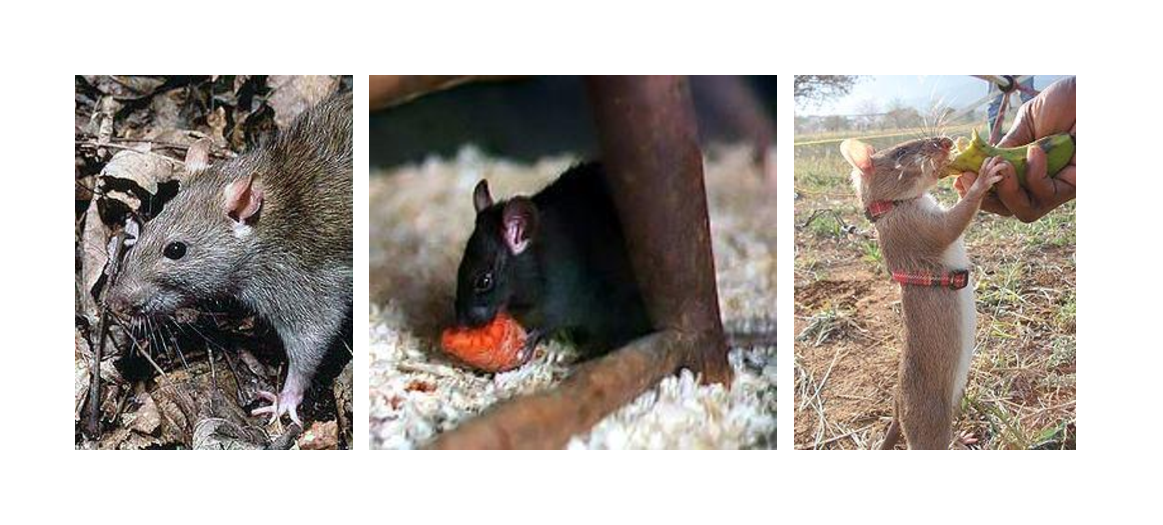
\includegraphics[width=6in,trim={0 .4in 0 .4in},clip]{RatVariations}
\caption{Left: Brown Rat (\textit{Rattus norvegicus})~\cite{BrownRatWikipedia2014}, Center: Black Rat (\textit{Rattus rattus})~\cite{BlackRatWikipedia2014}, and Right: Giant Pouched Rat (\textit{Cricetomys gambianus})~\cite{GiantPouchedRatWikipedia2014}\\
The three species pictured above are those that are discussed in this project. Note that while all three of these species are referred to as rats, as they all display characteristics associated with the term ``rat,'' only those two belonging to genus \textit{Rattus}, the brown rat and the black rat, are considered true rats.}
\label{RatVariationsFigure}
\end{figure}

How, then, are ``rats'' defined here? For the purpose of this project, the biological definition - where the term ``rat'' refers to members of the genus \textit{Rattus} - is generally used. However, a more specific definition of the term - strictly within the contexts of this project - is any animal that is a member of one of the following three species (Figure~\ref{RatVariationsFigure}):
\begin{enumerate}
\item Brown Rat (\textit{Rattus norvegicus}) - Also referred to as the common rat, the grey rat, the wharf rat, the Hanoverian rat or the Norway rat~\cite{Barnett1975, Barnett2001}, this species appears on every continent (with the exception of Antarctica) as a human symbiote, though it is suspected to have originated in northern China~\cite{WalkerRattus1999}. All domesticated rat strains - ``groups of individuals that share a presumed common ancestry and have clear cut physiological but not usually morphological distinctions''~\cite{Hanson2012} - are members of this species, and of the three species of rat discussed in this text, these share the closest connection to humans in the modern age. While the name is somewhat misleading (the ``brown'' rat is not always brown - tending, in fact, towards white and/or black in domesticated strains), this species is referred to as the brown rat throughout this project.
\item Black Rat (\textit{Rattus rattus}) - Also referred to as the old English rat, the blue rat, the roof rat, the Alexandrine rat, or the ship rat~\cite{Barnett1975, Barnett2001}, this species is present ``throughout Africa, southern Asia, Australia, and the southern coast of the United States''~\cite{ONeill} as a human symbiote, though is it likely originally native to India~\cite{WalkerRattus1999}. Until recently, when it was replaced by the brown rat, this species had the greatest impact on humans in Europe~\cite{Barnett2001}. This is the species most closely associated with, and in some sense responsible for, the Black Plague. As with the brown rat, while the name is misleading (the ``black'' rat is, in fact, very rarely black), this species is referred to as the black rat throughout this project.
\item Giant Pouched Rat (\textit{Cricetomys gambianus}) - Also referred to as the African giant pouched rat or the Gambian pouched rat~\cite{APOPO}. As the name implies, this species is large, weighing up to 1.5 kilograms, and has cheek pouches similar to a hamster~\cite{APOPO, WalkerCricetomys1999}. This species is not a true rat, but it does fit within the common definition of the term ``rat'' that has been established within the English language. While this species does not feature prominently in connection with human history, it does play an interesting role in current rat-human relations, and provides a case study with which to compare and contrast the main narrative presented here, and is therefore included in this project.
\end{enumerate}

Having established the definitions of the terms ``rat'' and ``human,'' the next necessary task is to clarify what is meant by the term ``co-evolution'' in this project.

\section{Co-Evolution and Reciprocal Adaptation} \label{Co-Evolution}

Throughout recorded history, there has been close contact between rats and humans. Because of this contact, it is not unreasonable to suggest that co-evolution occurred at some point. In order to isolate and analyze any possible occurrences, however, it is first necessary to define what, precisely, co-evolution is. Unfortunately, this can be a somewhat difficult task, as co-evolution is defined in a variety of different ways, depending on the circumstances. For example, in their essay titled ``Coevolution'' in the \textit{Encyclopedia of Biodiversity}, Futuyma and Levy define co-evolution as ``evolutionary changes in two or more different species owing to ecological interactions between them"~\cite{FutuymaLevy2001}. However, within this definition, Futuyma and Levy identify three separate contexts for interactions and four distinct potential formats of co-evolution. In order to examine the possibility of co-evolutionary processes between rats and humans, it is first necessary to identify where in the spectrum of possibilities this relationship lies.

The first factor of the co-evolutionary relationship as outlined by Futuyma and Levy is the interaction. Their definition describes three potential contexts for interaction:
\begin{enumerate}
\item Competition - ``[I]nteraction between individuals of the same or different species, whereby resources used by one are made unavailable to others''~\cite{FutuymaLevy2001}.
\item Mutualism - ``[S]ymbiotic relationship in which each of two species benefits from the interaction''~\cite{FutuymaLevy2001}.
\item ``Enemy/Victim'' Interactions - Including ``interactions between predators and prey, parasites and hosts, and herbivores and plants''~\cite{FutuymaLevy2001}.
\end{enumerate}
The rat-human interaction is interesting in that is displays elements from all three of these contexts. Rats and humans compete over food resources, although both rats and humans have diets that are significantly varied to the extent that if one species ``wins'' this competition, the loser can usually turn to alternative means of sustenance. Rats benefit from human technology and food stores, while humans benefit from studying rat anatomy in order to better understand their own (although this aspect of mutualism is a fairly recent development), and both animals are also capable of severely harming each other. Finally, while it may be argued that rats have a somewhat parasitic relationship to humans, living off their food and spreading disease, it could also be argued that humans have a predatory relationship with rats, turning to them for sustenance and using their bodies for research. From this, then, it is not unreasonable to conclude that the rat-human relationship fits into all of these contexts. This, however, is perhaps not quite as problematic as one may assume, as the more important feature in recognizing co-evolution is the process by which it occurs.

The second factor is the format the co-evolutionary process follows. Futuyma and Levy outline four possibilities:
\begin{enumerate}
\item Patterns of Correlated Evolution (Phylogenetic Congruence) - Occurs when ``the phylogeny of one clade of species... is congruent with that of a clade with which it interacts''~\cite{FutuymaLevy2001}. This is commonly demonstrated in the phylogenies of hosts and host-specific parasites. These patterns are considered co-evolution under the assumption that they occur as a result of interactions between the associated species. However, it is also possible that these patterns occur simply as a result of a ``shared history of geographical isolation''~\cite{FutuymaLevy2001}.
\item Reciprocal Adaptive Responses - This form of co-evolution is further divided into two sub-forms:
\begin{enumerate}
\item Specific Co-Evolution - ``[R]eciprocal adaptation of two species, independent of their interactions with other species''~\cite{FutuymaLevy2001}.
\item Diffuse Co-Evolution - ``[O]ccurs when evolutionary change in one species affects its interaction with two or more other species''~\cite{FutuymaLevy2001}.
\end{enumerate}
\item Co-Speciation - Occurs when new associated species develop as a result of the interaction between species. This, similar to correlated phylogenetics, often occurs in host and host-specific parasite interactions~\cite{FutuymaLevy2001}.
\item Escape-and-Radiate Co-Evolution - Occurs when ``an evolutionary lineage diversifies after it evolves a defense that breaks its association with enemies''~\cite{FutuymaLevy2001}. This form was first proposed in relationship to herbivorous insect/plant interactions~\cite{FutuymaLevy2001}, but could likely be extended to any other type of enemy/victim interaction.
\end{enumerate}
Here, it is much easier to categorize the rat-human relationship than before. There is certainly no indication of phylogenetic congruence between the two animals, considering there is 1 species of humans, and 56 species of rats. There is also little indication that the rat-human relationship has resulted in either co-speciation or escape-and-radiate co-evolution: while humans have domesticated the brown rat (as a laboratory or companion animal), this is not equivalent to the development of a new species, and humans, once again, are all defined within a single species. By process of elimination, this leaves reciprocal adaptive responses and specifically specific co-evolution. And, in fact, this seems to most accurately describe the interactions this project is examining.

However, determining whether or not rats and humans have undergone reciprocal adaptation is still difficult. As discussed by Futuyma and Levy, reciprocity is often difficult to determine:

\begin{quote}
``Often, the adaptation of one species to others is obvious, but reciprocal adaptation of the others is not. Because we seldom know a priori whether or not adaptation has been reciprocal, adaptations to ecological interactions are often loosely referred to as ``coevolutionary,'' even if evidence for reciprocity is slight or lacking. Certainly the study of coevolution includes adaptations to other species, which may or may not prove to have adapted in turn''~\cite{FutuymaLevy2001}.
\end{quote}

Additionally, the term ``adaptation'' is in and of itself a concept difficult to define. In \textit{Evolutionary Psychology}, Buss defines ``adaptation'' as ``an inherited and reliably developing characteristic that came into existence through natural selection because it helped to solve a problem of survival or reproduction during the period of its evolution''~\cite{Buss2004}. Additionally, the following three definitions of ``adaptation'' are both well accepted and usually conflated:
\begin{enumerate}
\item Adaptation is a trait that confers enhanced reproductive success to an individual in the present.
\item Adaptation is a trait that not only confers enhanced reproductive success to an individual in the present, but also did so in the past, and as a result is the product of natural selection.
\item Adaptation is a trait that conferred enhanced reproductive success to an individual in the past, but which may or may not confer enhanced reproductive success to an individual in the present, and may actually be maladaptive in the present.
\end{enumerate}
Therefore, in order to use reciprocal adaptation as evidence of co-evolution in rats and humans, adaptive changes in physiology and behavior resulting from natural selection must be demonstrated in these two species as a result of their interactions, and these adaptive changes must lead to enhances reproductive success in each species, either in the present or in the past. However, while co-adaptation is often accepted as proof of co-evolution in the absence of evidence to the contrary, it also must be noted that it is also possible for co-adaptation to occur as a result of two species developing traits independently of each other that just happen to make the species well adapted to each other~\cite{SparkNotes}.

Within this project, as a result, demonstrating co-evolution directly may not be possible. Therefore, this project will attempts to provide evidence for co-adaptation by examining the physical and cultural relationship between rats and humans.

\section{Taxonomy} \label{Taxonomy}

Before moving into an examination of the evidence indicating reciprocal adaptation between rats and humans, it is worthwhile to outline the taxonomies of these two species, and to examine the ways in which they are similar and dissimilar. This information is relevant, because it illuminates how rats and humans interact, and how each affects the other.

Rats and humans, as it turns out, are remarkably similar creatures at the biological level. To begin, first consider the eight major taxonomic ranks, and where rats and humans fit into this system:
\begin{enumerate}
\item Domain - The highest taxonomic rank. Rats and humans are classified within the domain \textit{Eukarya}: both have cells that consist of a nucleus and other organelles enclosed within a membrane.
\item Kingdom - The second highest taxonomic rank. Rats and humans belong to the kingdom \textit{Animalia}: both are animals; multicellular organisms with fixed body plans, capable of spontaneous, independent movement. Both must also ingest other organisms in order to survive.
\item Phylum - The third highest taxonomic rank. Rats and humans are members of the phylum \textit{Chordata}: both are vertebrates; they possess a spine and spinal cord.
\item Class - The fourth highest taxonomic rank. Rats and humans belong to the class \textit{Mammalia}: both are mammals. Both are warmblooded, give birth to live young, nurse young with breast milk, and possess hair/fur.
\item Order - The fifth highest taxonomic rank. At this point, rats and humans have separated. Rats belong to the order \textit{Rodentia}, while humans belong to the order \textit{Primates}. Rats, as rodents, have incisors that will grow continuously throughout their life. Rodents must gnaw in order to wear these incisors down; if not, their jaws would eventually lock together, either causing the animal to starve or the incisors to pierce the skull. Other commonly recognized characteristics of rodents are their short lifespan and rapid reproductive turnover, typically small size, and dependency on their strong sense of smell~\cite{WalkerRattus1999}. By contrast, humans, as primates, have a grasping ability attributable to the possession of opposable thumbs (most primates are also capable of grasping with their feet, but humans have lost this ability), possess large brains relative to body size, and have long lifespans with low reproductive turnover~\cite{Meek}.
\item Family - The sixth highest taxonomic rank. Rats are members of the family \textit{Muridae}, while humans are members of the family \textit{Hominidae}. Rats, as murids, are characterized by their slender bodies, scaled tails, whiskers, and pointed snouts. Rats also demonstrate the strong senses of hearing and smell and frequent breeding habits typical of murids. Humans, as hominids (commonly referred to as the ``Great Apes''), are bipedal and demonstrate an erect posture.
\item Genus - The seventh highest taxonomic rank. Rats are classified within the genus \textit{Rattus}, while humans are classified within the genus \textit{Homo}. Rats (or ``true rats''), as described in Section~\ref{Definitions}, are medium-sized murids with long, thin, hairless tails. Humans, also described in Section~\ref{Definitions}, are the only surviving species of the genus \textit{Homo}.
\item Species - The lowest taxonomic rank. There are many species within the genus \textit{Rattus} (though this project, as discussed in Section~\ref{Definitions}, is primarily concerned with two - the brown rat \textit{Rattus norvegicus} and the black rat \textit{Rattus rattus}), but only one extant species (\textit{Homo sapiens} or \textit{Homo sapiens sapiens}) within the genus \textit{Homo}.
\end{enumerate}
Rats and humans, therefore, split off below the class level into their respective orders, with their unity as mammals divided between rodents and primates. However, there are additional ranks interspersed among these main eight, and upon closer examination it is found that there is a rank between class and order where rats and humans are still linked. This is the clade, or the superorder, and both rats and humans are classified within the clade \textit{Euarchontoglires}. This rank indicates some of the most exclusive taxonomic characteristics that both species share; primarily, both have complex jaw muscles in order to control chewing.

Outside of those determined by their mutual taxonomy, rats and humans share many other similarities. Both are omnivores, and consume many of the same foods. Both also share the same basic physiology, and have similar organs and body plans~\cite{Spencer2012}. This similarity has significant impact on the rat-human relationship, which is discussed in greater detail later on in this project, and in particular in Subsections~\ref{Disease} and~\ref{Research}.

\section{History} \label{History}

At this point, it is now possible to begin to outline potential sources of evidence of reciprocal adaptation between rats and humans. The first such indicator examined is the representation of the rat in human culture.

Humans have immortalized the rat in literature, cultural traditions, and religious practices and teachings. Regardless of culture, much of this presents the rat as a creature to be feared and distrusted. Evolutionary psychologists suggest that because of human evolutionary history, certain environmental stimuli is inherently feared, resulting in phobias that currently persist in humans~\cite{Buss2004}. As a result, the consistency in the negative depiction of rats across cultures and throughout history may hint at the presence of an evolved psychological mechanism to fear or detest rats within the human brain. This section of this project documents the general opinion of rats that may be gathered from the accounts stemming from various human cultures (Figure~\ref{WorldMapFigure}).

This is, of course, by no means an exhaustive list of the cultures in which references to rats have appeared, and even for the limited list of cultures discussed within this section, the information presented is not by any means complete. Additionally, while some of these histories use the terms ``mouse'' or ``mice,'' in all likelihood they are actually referring to rats, based upon description, and, in fact, many ancient cultures did not have words to distinguish the two animals. The term ``rat'' itself did not exist in the English language until 1378~\cite{ONeill}. As a result, many early writings conflate rats, mice, voles, hamsters, and other small field and meadow dwelling rodents.
\begin{figure}
\centering

\includegraphics[width=6in,trim={0 .4in 0 .4in},clip]{WorldMap}
\caption{World Map~\cite{VisitedCountries2014}: Countries Discussed Marked in Red\\
Note: Some of the countries marked are approximations, rather than the exact locations of the cultures discussed. For example, modern Greece is marked, because ancient Greece is discussed. However, the influence of ancient Greece was geographically larger than modern Greece.}
\label{WorldMapFigure}
\end{figure}

\subsection{Religion} \label{Religion}

The history of religion and spirituality, interestingly enough, contains a wealth of information about how rats and humans have lived together in the past. This is because religion was and is a method of guiding human behavior in everyday life. Religious teachings and practices regarding rats, therefore, were usually implemented in order to educate practitioners on how to remain healthy and safe in regard to interactions with rats.

This subsection presents various accounts from religious texts and spiritual beliefs from a variety of cultures and countries.

\subsubsection{India} \label{India}

India is widely accepted to be the birthplace of the black rat (and potentially also the brown rat), and as such, it makes a certain amount of sense that possibly the oldest account of rats appears here. In the \textit{Atharva Veda}, a sacred Hindu text dating back to the second millennium BCE (possibly as early as the late third millennium BCE), there is a curse against rats: ``O, Ashwini. Kill the burrowing rodents which devastate our food grains, slice their hearts, break their necks, plug their mouths, so that they cannot destroy our food''~\cite{Barnett2001}.

Despite this threat of violence, the rat also makes an unexpected appearance as the companion of a Hindu deity. Ganesha, four-armed with the head of an elephant, is the god of literacy and learning. He is closely associated with rats~\cite{Barnett2001}. The significance of this is debated. One explanation is tied to the representation presented in the \textit{Atharva Veda}, with rat as destroyer. In this depiction, the rat is subservient to Ganesha, the destroyer conquered by the overcomer. An alternative viewpoint claims that the rat is a symbol, indicating that Ganesha is capable of appearing, like the rat, in even the most secret of places~\cite{Barnett2001}.

In the curse from the \textit{Atharva Veda}, rats are clearly negative. In relation to Ganesha, they take on a more neutral appearance. And finally, in the Karni Mata cult of a Jain temple in Deshnoke, Rajastan, can be seen a hint at the rat as positive. Here, rats are worshiped as ancestors~\cite{Edelman2005}.

In Indian culture, then, the rat is found in all three positions of negativity, positivity, and neutrality. A possible reason for this phenomenon is precisely because of the rats' origins in this country. Consider the following: much of the hatred, fear, and distrust of rats found throughout various human cultures stems from the rats' persistent interference in human lives and livelihoods: they spread disease, and eat or soil huge amounts of food intended for human consumption. But the rat, as an animal, evolved before the human, meaning that for at least some portion of its existence, it managed to survive \textit{sans} the convenience of human environments. Therefore, it could be argued that in the areas in which rats originated, humans were at first able to coexist peacefully with rats - the rat was just another animal. This could explain the neutral and even more positive representations of the rat in Hinduism and Jainism.

However, over time, the rats would have adapted to interacting with humans and their environments, coming to enjoy and even rely upon plentiful human food stores, and as the rat began to integrate itself into the human world, it took disease with it. Here, in the adaptability of the rat to human environments, there was a response in kind from humans, and the rat took on more negative connotations.

\subsubsection{France} \label{France}

Thousands of miles away, and many thousands of years later, in France, there is find an eerie echo of the \textit{Atharva Veda}, wherein the Bishop of Autun put rats under a formal curse~\cite{Barnett2001}. Attitudes, despite distance and time, had clearly not changed.

This fear of rats, however, does not seem to have prevented the French from eating them, not just as sustenance, but as delicacies. First published in 1938, the \textit{Larousse Gastronomique} provides directions on how to properly prepare rat flesh for gourmet consumption: skin and clean, then season with oil and shallots and grill over an open fire~\cite{Barnett2001}.

Here again is an account indicative of the reciprocal nature of the relationship between rats and humans. Between the time and place of the \textit{Atharva Veda} in India and that of the \textit{Larousse Gastronomique} in France, attitudes regarding rats had clearly not changed, despite vast differences in culture. This would indicate that as the rat spread across the planet, their reputation followed them. However, rats did not achieve a near global presence alone. It is highly likely that humans are most responsible for the current global distribution of their most hated adversaries.

Consider the following: in his paper ``Rats, Communications, and Plague: Toward an Ecological History,'' McCormick states that, because of the sedentary lifestyle of the rat, the average black rat will not travel farther than approximately 200 meters in its lifetime. If the average wild black rat lives to be two years old, then on average, it would therefore take a population of black rats approximately five generations - ``roughly, five years, depending on the ecological circumstances''~\cite{McCormick2003} - to move a kilometer, or approximately a century to move 20 kilometers~\cite{McCormick2003}. As McCormick describes:

\begin{quote}
``If this rate of self-powered locomotion is even remotely accurate, rats clearly did not traverse under their own power the more than 800 km from the Mediterranean coast to a first-century archaeological site at Baron, near Senlis, in only two to four centuries''~\cite{McCormick2003}.
\end{quote}

Here, then, in addition to a consistency in the perception of the rat across culture, is an indication that humans played a crucial role in the spread of the rat. Rats cannot travel large distances at high speeds, even if they were to deliberately try. Humans, on the other hand, can. And so the rat, following the food supplies it had previously so readily adapted to, now additionally adapted to human travel, and a variety of different environments.

\subsubsection{Israel} \label{Israel}

Finally, this project references text which would eventually be incorporated into sacred texts from three of the most widespread religions today: Judaism, Christianity, and Islam. Within the Bible (\textit{Leviticus} 11:1-47), the God of the Israelites provides a lengthy categorization of clean and unclean animals. A significant portion of this text is devoted to rats and related animals:

\begin{quote}
``Of the animals that move about on the ground, these are unclean for you: the weasel, \textbf{the rat}, any kind of great lizard, the gecko, the monitor lizard, the wall lizard, the skink and the chameleon. Of all those that move along the ground, these are unclean for you. Whoever touches them when they are dead will be unclean till evening. When one of them dies and falls on something, that article, whatever its use, will be unclean, whether it is made of wood, cloth, hide or sackcloth. Put it in water; it will be unclean till evening, and then it will be clean. If one of them falls into a clay pot, everything in it will be unclean, and you must break the pot. Any food that could be eaten but has water on it from such a pot is unclean, and any liquid that could be drunk from it is unclean. Anything that one of their carcasses falls on becomes unclean; an oven or cooking pot must be broken up. They are unclean, and you are to regard them as unclean. A spring, however, or a cistern for collecting water remains clean, but anyone who touches one of these carcasses is unclean. If a carcass falls on any seeds that are to be planted, they remain clean. But if water has been put on the seed and a carcass falls on it, it is unclean for you''~\cite{Leviticus1984}.
\end{quote}

Of the 47 verses that make up this chapter, it is worth noting that 9 (\textit{Leviticus} 11:29-38) are devoted specifically to rats and their equals in uncleanliness (quoted previously), and another 7 that may be applied to rats. The second largest count, at 7 verses (\textit{Leviticus} 11:13-19), applies to unclean ``birds'' (quoted next - note that the term ``bird'' refers here not strictly to birds, but to animals capable of flight), but notice that the content between the two is markedly different:

\begin{quote}
``These are the birds you are to detest and not eat because they are detestable: the eagle, the vulture, the black vulture, the red kite, any kind of black kite, any kind of raven, the horned owl, the screech owl, the gull, any kind of hawk, the little owl, the cormorant, the great owl, the white owl, the desert owl, the osprey, the stork, any kind of heron, the hoopoe and the bat''~\cite{Leviticus1984}.
\end{quote}

The section on birds is straightforward: here is a list of the birds that are unclean, do not eat them. The section which refers to rats and their counterparts is far more detailed: here is list of animals that are unclean, do not eat them and do not touch their carcasses; if you do, or if their carcasses come into contact with any of your possessions, here are the correct cleansing procedures. The threat level for rats is much higher.

It is often stated that the reasoning behind the categorization of animals into clean and unclean categories largely related to health concerns, and in particular dietary concerns. This however, does not explain the added emphasis for rats. A possible explanation, however, may be found on the level of contact. The birds listed above were mostly likely not a part of the daily lives of humans. Therefore, it was sufficient to simply say ``these are unclean, do not eat them,'' and leave the issue at that. Rats, on the other hand, probably were a constant presence. In this case, it would make sense that additional precautions be attached.

\subsection{Literature} \label{Literature}

In addition to religion, it is also possible to obtain hints as to the relationship between rats and humans through an examination of literature. This section will explore themes in literature and other writings taken from various cultures, and analyze what these stories may potentially reveal about the relationship between rats and humans.

\subsubsection{Greece} \label{Greece}

In Greece, it is claimed a farmer wrote the following note to the rats attacking his crops: ``I adjure you, ye mice here present, that ye neither injure me, nor suffer another mouse to do so. I give you yonder field. But if I catch you here again, by the mother of the gods, I will rend you in seven pieces''~\cite{Barnett2001}. This, again, echoes the curses of the \textit{Atharva Veda} and the Bishop of Autun.

\subsubsection{England} \label{England}

Much later, in England, rats were viewed as killers. The following passage from the George Orwell novel \textit{Nineteen Eighty-Four} is just one example of the fear that the rat inspired: ``a woman dare not leave her baby alone... even for five minutes. The rats are certain to attack it. Within quite a small time they will strip it to the bones''~\cite{Barnett2001}. But while there are various accounts of rats attacking humans, this is far from the norm (approximately 50000 people are bitten by rats each year~\cite{Sullivan2004} - out of a global population of 7.2 billion). While perfectly well adapted to live alongside human activity (as has been discussed extensively within this project), wild rats, like many other animals, have learned to fear humans. In principal, a wild rat will not approach a human.

However, rats were also recognized as having positive qualities. One account describes the compassion of rats for their own kind:

\begin{quote}
``Although its disposition appears to be naturally exceedingly ferocious... an anecdote [of a rat] exhibiting a degree of tenderness and care towards the disabled and aged members of their community... an old blind Rat, which held a piece of stick at one end in its mouth, while another Rat had hold of the other end of it, and thus conducted his blind companion''~\cite{Barnett2001, Marrin2006}.
\end{quote}

And, of course, regardless of whether the rat was a creature of good or evil, it was never a crime to use it for profit. During the fourteenth century, rat skins were sold for one farthing apiece~\cite{Barnett2001}. While the monetary value of a farthing only amounted to a quarter or a penny, this was, at the time, considered a useful amount. Later, in the 1800s, and possibly as early as the late 1700s, the popularity of ``rat baiting'' - a pub sport which consisted of emptying dozens of rats from sacks into pits, setting dogs on them, and spectators placing bets on how many rats the dogs could kill - provided plentiful income to ``rat catchers'' (these topics, and their impact on the domestication of the rat are discussed in further detail in Subsection~\ref{Companionship}).

The point is, at this location in time, humans began developing a slew of technologies for using rats to their advantage - whether that was to exterminate them or keeping or killing them for human amusement. This could possibly be viewed as an adaptation meant to once again give humans the upper hand in the relationship.

\subsubsection{United States}

When Europeans came to the United States, the rats followed. And with these rats came the European fear and disgust so closely associated with them. In the Edgar Allan Poe story \textit{The Pit and the Pendulum}, we find a passage that echoes the tone and emotion of \textit{Nineteen Eighty-Four} (quoted in previous subsubsection):

\begin{quote}
``They pressed - they swarmed upon me in ever accumulating heaps. They writhed upon my throat; their cold lips sought my own; I was stifled by their thronging pressure; disgust, for which the world has no name swelled my bosom and chilled, with a heavy clamminess, my heart''~\cite{ONeill}.
\end{quote}

The fear is evident in this passage; interestingly enough, however, it is through the work of the rats that the protagonist eventually narrowly escapes death.

However, it is also possible to occasionally find an undercurrent of human sympathy and compassion of the hated rat. For example, it is claimed that a farmer once wrote a letter to his rats, in a gesture which echoes the example presented from Greece, explaining that crops were short and that he could not afford to keep the rats during the winter, requesting that they take his neighbors' grain instead~\cite{Barnett2001}.

In the literature provided in these three examples, the rat, while still true to its past as an undesired thief, is also allowed some growth in personality. This may, in fact, also have been due to religion, in particular the popularity of Christianity. Regardless, of the cause, however, this indicated an adaptation, or perhaps a resignation, of humans to the presence of rats in their lives.

This, then, is a general overview of the histories of rats and humans. The next goal of this project is to extend the influence of this relationship into the present. In the last few centuries, the connection between rats and humans has taken on new layers. These dimensions are discussed in the following section.

\section{Current Cultural Identities of the Rat} \label{Identities}

In Section~\ref{History}, this project covered a handful of historical accounts of rat-human relationships. This section, in a sense, is merely a continuation of the previous. However, it has been separated, for two reasons.

First, there is the growing phenomenon of globalization. While historically, there were connections between cultures, through trade and other means, and these cultures did influence each other, for the most part various cultures were distinct and separate from one another. Today, however, this is becoming less and less the case, with such innovations as faster modes of transportation, and instant communication networks, including the internet. The aspects of the rat-human interaction discussed in this section are more recent, and therefore, are far more global in nature than connected to any specific locality.

Second, in the contemporary age, the rat can usually be categorized into one of three distinct identities, documented in \textit{Rats are People, Too!: Rat-Human Relations Re-Rated}. Here, Edelman argues that the modern rat has a ``triple identity'': the positive of rats as pets, the negative of rats as vermin, and the neutral of rats as laboratory animals~\cite{Edelman2002}. In this project, this break down is generally accepted, and these three categories are indeed presented and analyzed within this section.

\subsection{Vermin} \label{Disease}

First, there is the rat as vermin. Keep in mind, vermin, as defined by Merriam-Webster, are ``small insects or animals (such as fleas or mice) that are sometimes harmful to plants or other animals and that are difficult to get rid of''~\cite{MerriamWebster}.

Perhaps the most obvious reason for this categorization is the association in the human mind of rats with disease, an association that is, admittedly, not entirely undeserved. In \textit{Rats: Observations on the History and Habitat of the City's Most Unwanted Inhabitants}, Sullivan describes the involvement of the brown rat in spreading disease:

\begin{quote}
``They carry diseases that we know of and they may carry diseases that we do not know of - in just the past century, rats have been responsible for the deaths of more than ten million people. Rats carry bacteria, viruses, protozoa, and fungi; they carry mites, fleas, lice, and ticks; rats spread trichinosis, tularemia, leptospirosis. They carry microbes up from the underground streams of sewage; public health specialists sometimes refer to rats as ``germ elevators''''~\cite{Sullivan2004}.
\end{quote}

While this statement should be acknowledged with some skepticism - Sullivan does not provide any support for his data - it does give an idea of the magnitude of the issue. In a more specific example, rats are often blamed as the source of one of the ``deadliest epidemiological disasters of human history''~\cite{ONeill}. This disease was the bubonic plague, commonly known as the Black Death, which spread across Europe from 1347 to 1351, killing one in every three people~\cite{Gottfried1983}. And to an extent, it is true; the disease originated in the rodent populations. But the rats themselves were not immune; on the contrary, they were the first to die. When the rat population became depleted, the fleas that carried the disease sought human hosts and transferred the disease from rat to human~\cite{Marrin2006, ONeill}. Therefore, while rats certainly played a role in plague transmission, it is unfair and untrue to place all the blame on the shoulders of rats.

However, the bubonic plague does tell another story, in that is provides some evidence of co-evolution (or reciprocal adaptation) between rats and humans. This evidence stems from the almost complete disappearance of the bubonic plague from the late seventeenth century onward. One theory as to why this occurred (out of many) is that some rats developed immunity. Following the principles of evolution, then, ``most of the non-resistant rats may have died leaving only resistant rats''~\cite{Appleby1980, ONeill}. And, if the new populations of immune rats were not dying, the fleas that transferred the plague from rat to human had no reason to seek out new (human) hosts~\cite{ONeill}.

If we step backwards in time, we will find that the spread of the plague tended to follow trade routes. This makes sense, because the food that was moved along these routes would have attracted rats, at least some of which would have been infected. The rats would then settle in massive nests in European settlements, attracted by the squalid living conditions in medieval Europe. Under these circumstances, the fleas moved freely from rat to rat, quickly infecting most of the population. When the rats had died, the fleas turned to human hosts. In order to survive among humans, where conditions were for the most part favorable, it was therefore in accordance with the logic of evolution for the rat to develop immunity to the plague~\cite{ONeill}. And, as it happened (assuming this theory to be true), this development proved to be favorable for humans as well.

Interestingly enough, the same concept may also be applied to humans. Rats, by this point, were an inescapable part of everyday life in Europe. And with rats came the plague. If humans were to survive the plague, they needed to develop immunity. If certain humans were or became immune to the plague, these were the ones to survive, while the rest of the population died off. With mostly or only resistant humans left, the plague would have run its course. In all likelihood, a complete picture of the disappearance of the plague would include both scenarios. Therefore, if both rats and humans underwent natural selection as a result of the plague, there is evidence here for co-evolution, or at least reciprocal adaptation.

The second example is in the extent of human food losses incurred by rats, documented in the following passage:

\begin{quote}
``Conservative estimates have previously indicated that one fourth of the world’s food supply is damaged annually by rats, and recent evidence from Turkey suggest that rats help consume up to fifteen percent of Turkey’s grain and legume storage. Prosperous and food-rich nations, such as America, suffer high losses because of the rats. In one estimate, food losses incurred due to rats cost almost nineteen billion dollars a year for Americans. In America, the costs are largely monetary, as food supplies are too massive to be consumed in their entirety. On the contrary, small island nations struggling against Malthusian limits face far greater peril when confronted with the bottomless appetite of the rat''~\cite{ONeill}.
\end{quote}

And Sullivan adds further substance to this claim: ``Though targeted over and over by man, rats generally wreak havoc on food supplies, destroying or contaminating crops and stored foods everywhere. Some estimates suggest that as much as one third of the world's food supply is destroyed by rats''~\cite{Sullivan2004}.

Rats have taken advantage of the vast and consistent food supplies readily available through living in close contact with humans. This manifests itself in their continued reliance on human food sources, and in their capacity to decimate biodiversity within fragile ecosystems in situations where they are introduced and then left to their own devices~\cite{ONeill}.

However, there is a third reason behind the view of rat as vermin, in this case far more abstract. The brown rat is believed to have arrived in England in 1728, and to have completed its spread across the country by 1800 (note that the brown rat here displaces the previously well established black rat)~\cite{Edelman2002}. During the early 1800s, it is argued, the image of the rat went through a transformation, from ``despised'' to ``disgusting''. Previously, the rat had merely been a nuisance: invading houses and barns, and eating and soiling food intended for human consumption. With the development of the sewer system, however, the rat became synonymous with dirt and refuse, thereby making it abhorrent. The sewer became a physical underworld, intended to hide filth from sight and smell. The rats, which happily and readily entered into this underworld, were similarly rejected~\cite{Edelman2005}.

Interestingly enough, it is during this same period, when the rat is being transformed from a ``despised'' animal to a ``disgusting'' animal, that the two other primary identities of the rat, as laboratory animal and as pet, came into existence. These simultaneous occurrences are explored in the following two subsections.

\subsection{Laboratory Animal} \label{Research}

Second, there is the rat as laboratory animal. The first documented experimentation on rats dates back to 1856 in France, followed closely over the next few decades by experiments in England, Germany, and the United States~\cite{Edelman2002}. It is interesting, however, to note that experiments were occurring alongside the transformation of the rat from ``despised'' to ``disgusting,'' a process covered in the previous subsection.

One possible explanation is that the rat was chosen for experimentation simply because of its lowly status. In England, human dissection was prohibited until the 1500s, and was still largely limited and taboo until the first half of the 1800s. However, the human was, according to the England, separate from the animal: the human had a soul. Therefore, rats, as soulless animals, and low status animals at that, were free game.

Another explanation is the physical and economic advantages of the rat. Rats were small, easy to handle and reproduce, fairly low maintenance, quick to mature, and had short lifespans~\cite{Edelman2002}. These qualities well suited the rat to use in experiments and the laboratory environment.

Whatever the reason, the choice of rat as laboratory animal turned out to be a wise one, as rats and humans share a remarkable number of physical similarities, discussed previously in Section~\ref{Taxonomy}. Both species share similar organs, body plans, hormones, reproductive physiology, dietary habits, and aging processes. And, as a result, both are susceptible to many of the same diseases and other issues, which makes the rat an excellent subject for medical research.

For example, by implanting cancer cells in rat bodies, humans are better able to understand how cancer roots and spreads in human bodies. By exposing rats to tobacco smoke, a correlation was made between tobacco smoke and lung cancer. By testing anti-rejection drugs on rats, researchers have been able to save the lives of many surgical patients. Similarly, by testing vaccines on rats for treatment of certain diseases, researchers are better able to understand how the drugs will effect humans, to know whether they with help or hurt~\cite{Marrin2006}.

Here, then, in the rat as laboratory animal, there is an interesting dynamic, with humans using rats as a form of technology by taming and domesticating them for human use.

\subsection{Pet} \label{Companionship}

Third and finally, there is the rat as pet. And, as with the appearance of the laboratory rat, this identity began to form at approximately the same time the rat was being redefined from ``despised'' to ``disgusting.''

As briefly mentioned previously in Subsubsection~\ref{England}, during the middle of the 1800s, the sport of ``rat baiting'' became fashionable. While the practice was fairly short lived, it did provide ``rat catchers'' with an extra source of profit, in addition to their traditional role as exterminators. However, particularly innovative rat catchers discovered yet another means of making a profit off their chosen profession.

Some rat catchers, including ``Her Majesty's Rat Catcher'' Jack Black, discovered that they could breed rats for color and temperament, and sell these specimens, primarily to upper class women, for a relatively high price. To the rat catchers, the rat was solely a source of income; there was no sentimental value attached to them, no concept of them as living, feeling beings. But for the women who chose to purchase them, they were pets, companions, and even friends~\cite{Edelman2002, Edelman2005}. As a self-identified ``crazy rat lady'' writes:

\begin{quote}
``They [the rats] are very playful, playing the attack rat, jumping, popping up in the air, playing Boo with me, pretending to run away, only to quickly turn back thinking they fooled me. I love their wet cold noses. They are alive and can think, comfort you when sad, make you laugh, lave little hands with fingers to reach out to you. They make me feel loved and when all is calm and quiet and they're in my lap and I can feel their warm breath on my skin, I cannot express the feelings I get''~\cite{Edelman2005}.
\end{quote}

But how did this attitude come to exist? The perspective of the rat catchers fits within the idea of the rat as ``disgusting.'' This is not so for the rich women who kept these animals as pets. However, as with the previous identities of the rat discussed within this project, there are multiple possible explanations.

The first explanation is as simple as separation. These women had little to no contact with the ``disgusting'' sewer rat, and therefore, to their eyes, the rat could simply exist as yet another animal, even a lovable, adorable, and charming one.

A second explanation is also based in separation, but at a different level. In this scenario, the woman recognizes her pet rat as belonging to the same species as the ``disgusting'' rat, but to her, the individual triumphs over the group. As an example, the lower classes were often categorized in a similar manner to the rats: this was a group to be looked down upon, and viewed with disgust. However, just because the group was ``disgusting'' did not bar the individual from redemption. In this respect, the rats were to the women as Eliza is to Professor Higgins in \textit{Pygmalion}, a charming ``oddity'' of sorts~\cite{Edelman2002, Edelman2005}.

A third explanation is yet again based in separation, albeit again of a different variety. Here, the pet rat is still very much a member of its breed; at its core, it is still the ``disgusting'' sewer rat. But it is also only a single rat, separate from the horde. On it own, the positive qualities of the individual rat are now visible~\cite{Edelman2005}.

The fourth and final explanation presented in this project stands apart from its predecessors, in that its basis is not in separation, but in connection. Here, the pet rat is still very much a low, filthy, and even masculine creature. In keeping the rat, then, these women aimed to establish an identity, even status, for themselves, separate from that assigned them by their gender and class~\cite{Edelman2005}.

In support of this fourth explanation, and as a final note, in recent years, the rat has also achieved some popularity as a status symbol. Individuals identifying within certain subcultures, such as punks or goths, may opt to keep rats as pets precisely because of their association with the low, the filthy, and the frightening~\cite{Edelman2005}.

In its role as companion animal, the brown rat has succeeded in altering the human perception of its species. This, in turn, affects not only how humans treat domesticated rats, but wild rats as well. And as human treatment of the wild rat changes, so do the means by which it exists within the human world. As pet, then, the rat does not bring about biological adaptation so much as cultural adaptation, as both animals learn to interact with one another in new ways.

\section{Case Study} \label{Service}

This project has thus far documented rat-human interactions, and the implications these interactions have for determining the possible reciporcal adaptation between these species. In closing, this project outlines a contemporary case study of the connection between the giant pouched rat and humans.

The primary point of reference for the connection between giant pouched rats and humans is the HeroRAT - a giant pouched rat trained by the organization APOPO (Anti-Persoonsmijnen Ontmijnende Product Ontwikkeling - translated to English as Anti-Personnel Landmines Detection Product Development). APOPO trains giant pouched rats - note that this species is an example of a case where the term ``rat'' is not applied to a true rat, but rather a rodent that demonstrates characteristics humans associate with the term ``rat'' - to detect land mines and, in more recent work, tuberculosis~\cite{APOPO}.

Why giant pouched rats? APOPO lists the following reasons:
\begin{enumerate}
\item Exceptional Sense of Smell - Rats may have up to 1000 different types of olfactory receptors, each coded for by a separate gene. This information alone takes up approximately 1\% of the total genetic code~\cite{Hanson2012}.
\item Intelligent and Trainable - APOPO also mentions, in relation to this information, that the giant pouched rat may have a lifespan of up to eight years, meaning that the rats live long enough to be productive.
\item Too Light to Set Off Mines - Giant pouched rats typically weigh about one kilogram, while anti-personnel landmines usually require a weight of about five kilograms to detonate. According to APOPO, a rat has never been injured or killed in the minefield.
\item Locally Sourced and Widely Available - APOPO currently has anti-personnel landmine detection and removal programmes in Tanzania, Mozambique, Thailand, Angola, Cambodia, Vietnam, and Lao PDR; and tuberculosis detection programmes in Morogoro, Tanzania; Dar es Salaam; Tanzania and Maputo, Mozambique. Giant pouched rats are native to three of these countries (and all three cities), and therefore adapted to function within the environment.
\item Easily Transferable Between Trainers - Rats do not tend to bond with particular humans, and so it is easy to move them to various locations as necessary.
\item Low Maintenance Cost - Rats are cheap to feed, train, transport, and breed.
\item Resistant Species - Giant pouched rats are native to Sub-Saharan Africa and are resistant to many potentially detrimental environmental factors in the countries in which they are used.
\end{enumerate}

Here, we see a use of rats in a very similar way to that established for the category of the rat as laboratory animal, with humans using rats as a form of technology. However, although the laboratory animal is readily sacrificed for the benefit of humans, the HeroRAT is largely protected from harm. APOPO dedicates a whole section of its Frequently Asked Questions page to ``Animal Welfare,'' and here, in response to the question ``Do animals sometimes get hurt or killed during the mine action job?,'' APOPO provides the following response:

\begin{quote}
``De-mining is a dangerous job and, sadly, human de-miners are sometimes injured or killed. The rats have a significant advantage over their human de-mining partners in that a pressure-activated antipersonnel land mine typically requires about five kilograms of pressure to be activated. Our heaviest operational male rats do not exceed 1.5 kilograms and are, therefore, in no danger of activating this type of land mine. However, working around land mines is dangerous work for anyone involved. Fortunately, no rats have been injured or killed in the minefield to date''~\cite{APOPO}.
\end{quote}

Clearly, then, the HeroRAT is not to be harmed. This indicates that the HeroRAT has a ranking somewhere above the laboratory animal, in that it is assigned the right to its own existence. Thus it is an animal that lies somewhere between the pet and laboratory animal, although in its native habitat it is considered vermin.

Like the black and particularly brown rat, the giant pouched rat is at once vermin, pet, and laboratory animal. And, again similar to their counterparts, these identities allow it to interact with the human on a variety of different levels, which in turn creates a web of possible exchanges in adaptation between the two species.

\section{Conclusions} \label{Conclusions}

Rats and humans share an extensive and complex history. The purpose of this project was to examine this history, and to attempt to understand the ways in which it has affected the two animals, particularly in a possible co-evolutionary sense.

In attempting to complete this objective, this project has documented the taxonomic similarities and differences between the rat and the human, the histories of these two animals throughout a number of world cultures, and the contemporary development of the various identities of the rat.

However, it is still difficult to prove co-evolution, or even reciprocal adaptation. Rather, these final paragraphs describe what can be concluded: that rats, as a species, are highly adaptable and used humans and human resources to their advantage; humans, as a species, are highly adaptable and adjusted to and even took advantage of the inescapable presence of rats; and a few of these adaptations may have happened in direct response to one another. The next few paragraphs will describe these conclusions individually.

First, rats are highly adaptable, and used humans and human resources to their advantage. This has been documented:
\begin{enumerate}
\item Resources - Rats existed long before humans. However, once humans had established themselves, rats came to enjoy and even rely upon access to human resources, and in particular the plentiful food availability. The contradictory portrayals of rats in Indian culture - where the black rat is believed to have originated - may possibly be a result of this change from the rat as just another animal to the rat as a constant nuisance. It may also in part explain the devastation rats may cause to isolated ecosystems into which they have been - either purposely or inadvertently - introduced: after coming to expect a plentiful food supply, when left to their own devices rats will do their best to continue this level of food intake.
\item Distribution - It is improbable that rats would spread as far and as fast as they did by their own means. It is likely that they achieved their current global distribution by means of human transport. Once arrived at their destination, the adaptability of the rat - and its continued access to human resources - allowed it to inhabit a variety of environments.
\end{enumerate}

Second, humans are highly adaptable, and adjusted to and even took advantage of the inescapable presence of rats. This too has been documented:
\begin{enumerate}
\item Culture - Negative attitudes toward rats are almost universal. This may be an indication of an instinctual fear that has been ingrained in human psychology as a result of evolution.
\item Technology - Humans have developed a variety of technologies in response to the presence of rats. Extermination is perhaps the most obvious example, of which the English rat catchers discussed in this project are just one case. Throughout history, humans have developed a variety of tactics for eliminating rats (while rats, in turn, have developed a variety of tactics for avoiding elimination), and even today, rat extermination is a profitable business. But humans have also domesticated the rat, as both a laboratory animal and a pet. As the former, rats have been used in a variety of medical advances, and as the later, rats have altered the human perception of and relationship to rats.
\end{enumerate}

Third and finally, some of the adaptations rats and humans have undergone may have happened in direct response to one another. The most notable example of this covered in this project is the Black Death. In order for both species to survive the plague, it is likely that both species had resistant members. Following the logic of natural selection, these resistant individuals would have survived and reproduced, while the rest died off. This, it seems, could potentially be definitive proof of co-evolution between the two species. However, this project has not covered this topic extensively enough to make this claim without reservation.

Both rats and humans are highly adaptable species, and share a close relationship. As a result, some of these adaptations appear to be in response to one another, and could perhaps be qualified as reciprocal adaptation, in which case co-evolution could be claimed. However, it is also a possibility that these adaptations occurred independently. Therefore, it will merely be claimed here that rats and humans are highly adaptable, and that this adaptability has allowed both species to adjust to and even benefit from the presence of the other. Further research on the Black Plague and how it affected both rats and humans could possibly provide a more definitive answer.

\section{Acknowledgments}

Thanks to Leslie Meek for acting as faculty advisor for this project, to Rebecca Dean and Heather Waye for acting as faculty panel members, and to all three for providing indispensable resources and advice.

\pagebreak

\bibliographystyle{acm}
\bibliography{StoryOfRatsBibliography}

\end{document}